% !TeX spellcheck = en_US
\documentclass[a4paper,12pt]{article}
\usepackage[utf8x]{inputenc}
\usepackage{wrapfig}
\usepackage{graphicx}
\usepackage{float}
\usepackage{listings}
\usepackage{amsmath}
\usepackage{caption}
\usepackage{subcaption}
\usepackage[usenames,dvipsnames,svgnames,table]{xcolor}
\usepackage{datetime}
\usepackage{fancyhdr}
\usepackage{multicol}
\usepackage{hyperref}
\pagestyle{fancy}

% Title Page
\title{Project1}
\author{Andreas Ellewsen, Peder Forfang}

\fancyhead[L]{Andreas Ellewsen, Peder Forfang }
%\fancyhead[C]{Solving Poisson equation numerically}
\fancyhead[R]{Fall 2015}

\begin{document}
\maketitle
\tableofcontents
\newpage
\%begin{multicols}{2}
\section{Introduction}
In this project we use various vector and matrix operations to solve the one dimensional Poisson equation with Dirichlet boundary conditions, such that $u(0) = u(1) = 0$.
\[
-u''(x) = f(x)
\]
for $ x ~\epsilon ~[0,1]$.
Since we want to solve this numerically the second derivative $u$ is approximated with
\[
   -\frac{v_{i+1}+v_{i-1}-2v_i}{h^2} = f_i  \hspace{0.5cm} \mathrm{for} \hspace{0.1cm} i=1,\dots, n,
\]
where $f_i=f(x_i)$, $x_i = ih$ and $h = 1/(n+1)$.

This is done using 3 different approaches. First a specialized Gaussian elimination, secondly a generalized Gaussian elimination, and finally LU decomposition. All three approaches are programmed in c++, and plotted using python.
The vector and matrix operations are imported from the Armadillo library for c++, and plotting of the solution is done using matplotlib in python.

To test our method we use a source function $f(x) = 100e^{-10x}$, and keep the same interval and boundary 
conditions. The above differential equation then has a closed-form  solution given by $u(x) = 1-(1-e^{-10})x-e^{-10x}$.

This is used to calculate the relative error for a number of different steplengths.

In the following report we describe our approach to the problem followed by our results and conclusion.

\section{Theoretical models and technicalities}
To solve this using linear algebra we first need to rewrite our equation as a matrix equation. To see how this can be done we write out the lines for $i = 0,1,2$ of the discretized approximation:
\[
2v_{0}       - v_{1} = h^2f_0  
\]
\[
-v_{0} +2v_{1} - v_{2} = h^2f_1  
\]
\[
-v_{1} + 2v_{2} -  v_{3} = h^2f_2  
\]
Looking at this it is easy to see that this can be written
\[
   {\bf A}{\bf v} = \tilde{{\bf b}},
\]
where 
\begin{equation}
    {\bf A} = \left(\begin{array}{cccccc}
                           2& -1& 0 &\dots   & \dots &0 \\
                           -1 & 2 & -1 &0 &\dots &\dots \\
                           0&-1 &2 & -1 & 0 & \dots \\
                           & \dots   & \dots &\dots   &\dots & \dots \\
                           0&\dots   &  &-1 &2& -1 \\
                           0&\dots    &  & 0  &-1 & 2 \\
                      \end{array} \right)
\end{equation}
and $\tilde{b}_i=h^2f_i$.

\subsection{Specialized Gaussian elimination}
To solve this in c++ we rewrite $\bf A$ into three vectors $\bf a$, $\bf b$, $\bf c$,
where $a_i = c_i = -1$, and $b_i = 2$. As in Gaussian elimination we proceed with a forward substitution, resulting in the following algorithm.
\begin{verbatim}
    for(int i=0 ; i <= n-1 ; i++){
        b[i+1] = b[i+1]*b[i] + c[i];
        c[i+1] = c[i+1]*b[i];
        b_tilde[i+1] = b_tilde[i+1]*b[i] +b_tilde[i];
    }
    b[n+1] = b[n+1]*b[n] + c[n];
\end{verbatim}
Note that we don't bother changing any of the a-values since they are not used more than once, and this would waste computation time. 
The next step is to do a backward substitution. In c++ this is implemented using the following algorithm.
\begin{verbatim}
     for(int i=n ; i >=0 ; i--){
        b_tilde[i] = b_tilde[i] - b_tilde[i+1]*c[i]/b[i+1];
     }
\end{verbatim}
By the same logic as above, we don't bother saving the c-values after they've been used.
It should also be noted that by rewriting $\bf A$ in terms of $\bf a$, $\bf b$, $\bf c$, the number of floating point 
operations is reduced substantially, since one no longer has to do calculations on all the elements in $\bf A$ that are zero.

The solution $v$ can then be extracted:
\begin{verbatim}
    for(int i=0; i<=n+1; i++){
        v[i] = b_tilde[i]/b[i];
    }
\end{verbatim}

\subsection{Relative error}
To test the precision of our method we also calculate the relative error.
\[
   \epsilon_i=log_{10}\left(\left|\frac{v_i-u_i}
                 {u_i}\right|\right),
\]
This is calculated for all i, and the largest value is kept for each $n = 10,100,1000,10000$, and $10^5$
The results are tabulated in table \ref{errortable}.


\begin{table}[H]
\begin{center}
\begin{tabular}{ | l | l |}
    \hline
    n      & rel. error \\ 
    \hline
    10     & 0.316526 \\  
    100    & 0.0384981 \\
    1000   & 0.00394574 \\
    10000  & 0.000395576 \\
    100000 & 3.95677e-05  \\
    \hline
\end{tabular}
\caption{Table of the relative error for different n}
\label{errortable}
\end{center}
\end{table}

The relative error decreases as n increases. This is expected because shorter steplength gives a closer approxiation to the analytic solution. Results in the table shows that the relative error is almost proportional to $h$ which is a good indication the code runs as it should.

\section{Results}
Comparing our method with the gaussian elimination and LU decomposition methods found in the armadillo library for c++, we find that the total floating point operations(flops) as well as the relative error is improved.
Counting the number of flops shows that the specialized method uses $8n$ flops, while the general method uses $3/2\times n^3+n^2$ flops, and LU decomposition uses $n^3$ flops. The totalt number of flops for the different methods using different can be seen in table \ref{flops}.

\begin{table}[H]
\begin{center}
\begin{tabular}{ | l | l | l | l |}
    \hline
    n      & SGE & GE & LU\\ 
    \hline
    10     & 80 & 1600 & 1000\\  
    100    & 800 & 1.51e+06 & 1e+06\\
    1000   & 8000 & 1.501e+09 & 1e+09\\
    10000  &  80000 & 1.5001e+12 & 1e+12\\
    \hline
\end{tabular}
\caption{Number of floating point operations for different methods and n.}
\label{flops}
\end{center}
\end{table}

\begin{table}[H]
\begin{center}
\begin{tabular}{ | l | l | l |}
    \hline
    n      & SGE & LU\\ 
    \hline
    10     & 6e-06 & 2.8e-05\\  
    100    & 2.2e-05 & 0.000902\\
    1000   & 0.000186 & 0.048007\\
    10000  &  0.001291 & 4.33961\\
    \hline
\end{tabular}
\caption{Time elapsed compared with LU decomposition in seconds}
\end{center}
\end{table}

Clearly the specialized method is the best solution when considering the time used. Our attempt to run the standard LU decomposition with $10^5\times10^5 $ failed misserably. This can be attributed to the fact that we are trying to save $10^{10}$ elements, each taking up 8 bytes, which exceeds the 8GB of ram available to the computer used for the calculations. This is where the difference between the two methods becomes apparent. The specialized method could easily run with higher n since that only needs $5n$ elements, while LU needs $n^2 +2n$ elements.

Looking at the plots reveals that the specialized method approaches the exact solution before the other methods.
Note that the line for LU decomposition lies exactly underneath the line for general gaussian elimination.
\begin{center}
\begin{figure}
 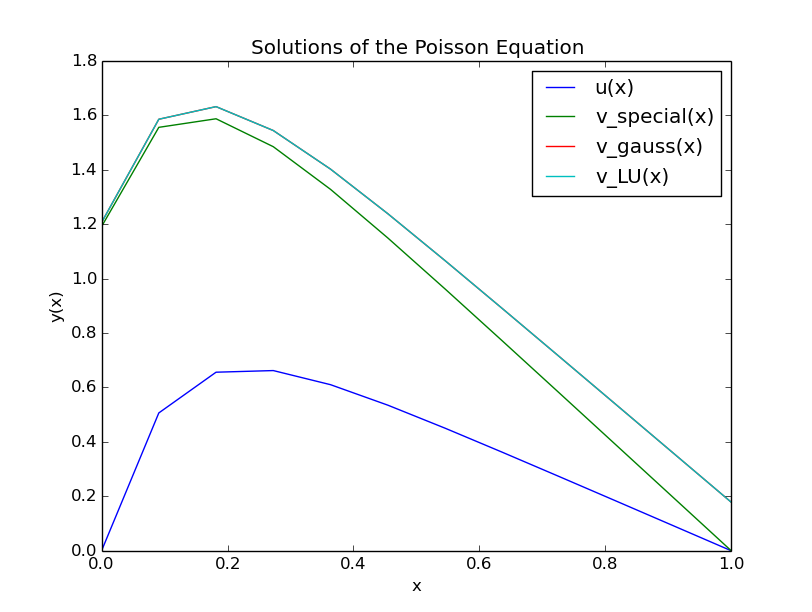
\includegraphics[width=.49\textwidth]{figure_n10.png}
 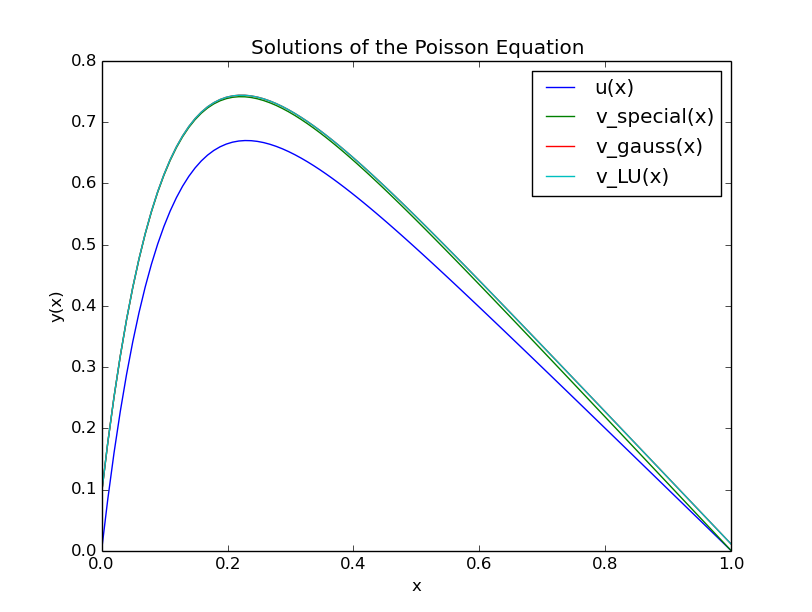
\includegraphics[width=.49\textwidth]{figure_n100.png}
 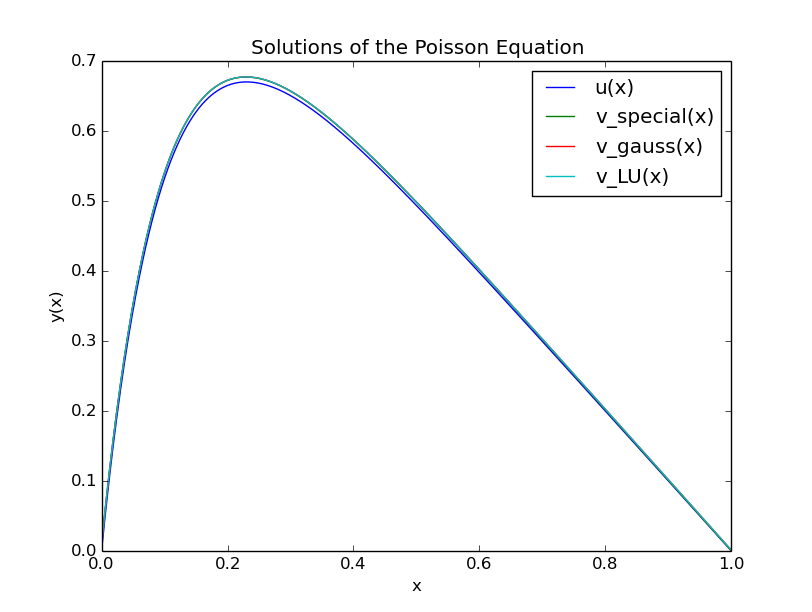
\includegraphics[width=.49\textwidth]{figure_n1000.png}
 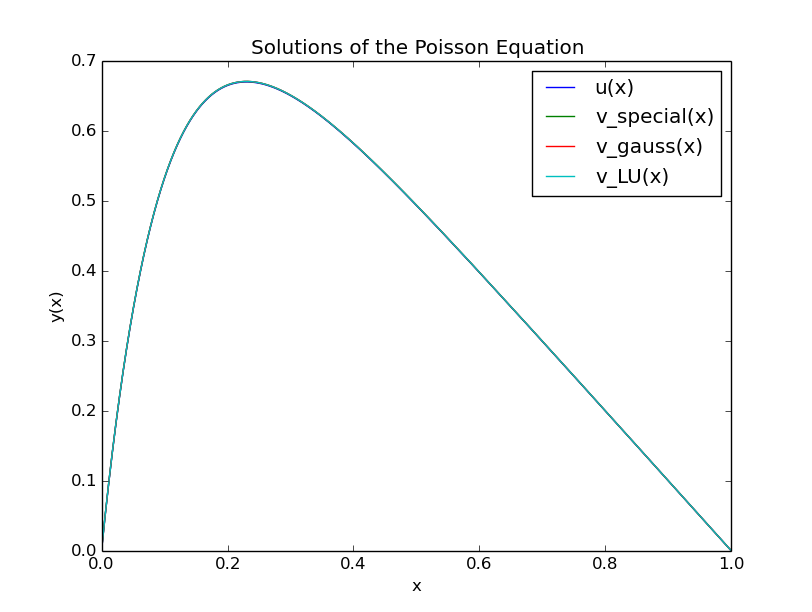
\includegraphics[width=.49\textwidth]{figure_n10000.png}
\caption{Plots of solutions with different methods for n = 10, 100, 1000, 10000 respectively.}
 \end{figure}
\end{center}
\newpage
\section{Conclusion}
Due to sloppy reading from the lecture notes, we both overlooked the fact that the algorithm was right there. We used alot of time making a spesialized method, which seemed wasted. However the learning process was greatly increased this way, and we have no regrets. After finishing this project, we both feel much more comfortable programming with C++. 
We also saw that taking the time to make a specialized solution to the problem at hand can greatly reduce the time it takes to make a numerical approximation, and allows for better precision by reducing the number of operations required.
%\end{multicols}
\section{Source code}
The source code for this document, the c++ project, and the python file for plotting can be found at \url{https://github.com/tellewsen/Project1}

\end{document}
